\documentclass[]{article}
\usepackage{amsmath}
\usepackage{amssymb}
\usepackage{stmaryrd}
\usepackage{latexsym}
\usepackage{graphicx}
\usepackage{fancyhdr}
\usepackage{color}
\usepackage{listings}
\usepackage[top=1in, right=0.75in, left=0.75in]{geometry}
\usepackage[colorlinks=true, linkcolor=blue]{hyperref}

\author{
	Mohammad Hossein Shafizadegan\\
	99104781
}
\title{
	Final Project \\
	Computational Intelligence  \\
	Dr. S. Hajipour
}

\pagestyle{fancy}
\rhead{CI}
\lhead{Project}

\newcommand{\pict}[2]{\begin{center}
		\includegraphics[width=#1\linewidth]{Fig/#2.png}
\end{center}}
\newcommand{\mat}[1]{\begin{bmatrix} #1 \end{bmatrix}}
\newcommand{\deter}[1]{\begin{vmatrix} #1 \end{vmatrix}}

\definecolor{customgreen}{rgb}{0,0.6,0}
\definecolor{customgray}{rgb}{0.5,0.5,0.5}
\definecolor{custommauve}{rgb}{0.6,0,0.8}

\definecolor{dkgreen}{rgb}{0,0.6,0}
\definecolor{gray}{rgb}{0.5,0.5,0.5}
\definecolor{mauve}{rgb}{0.58,0,0.82}

\lstset{frame=tb,
	language=MATLAB,
	aboveskip=3mm,
	belowskip=3mm,
	showstringspaces=false,
	columns=flexible,
	frame=single,	                   % adds a frame around the code
	basicstyle={\small\ttfamily},
	numbers=none,
	numberstyle=\tiny\color{gray},
	keywordstyle=\color{blue},
	commentstyle=\color{dkgreen},
	stringstyle=\color{mauve},
	breaklines=true,
	rulecolor=\color{black},
	breakatwhitespace=true,
	tabsize=3,
	numbers=left,                    % where to put the line-numbers; possible values are (none, left, right)
	numbersep=10pt,                   % how far the line-numbers are from the code
	numberstyle=\tiny\color{customgray}, % the style that is used for the line-numbers
}

\begin{document}
	\begin{figure}
		
\includegraphics[width=0.25\textwidth]{Fig/Sharif.png}
		\centering
	\end{figure}
	\maketitle
	\tableofcontents
	\newpage
		%-----------------------------------------------------------------------------------------------------------------	
	\section{Overview}
	The task played for the subjects consists of trials of video played by VR headsets. Videos contain positive and negative sentiments which are indeed our target of prediction. The provided dataset contains recordings of 59 electrodes, with sampling rate of $1 \,\, kHz$. The provided data is epoched 1 second pre-stimulus and 4 seconds post-stimulus. The total number of trials is 550. Here there is an overview of the data used in this project.
	
	\begin{center}
		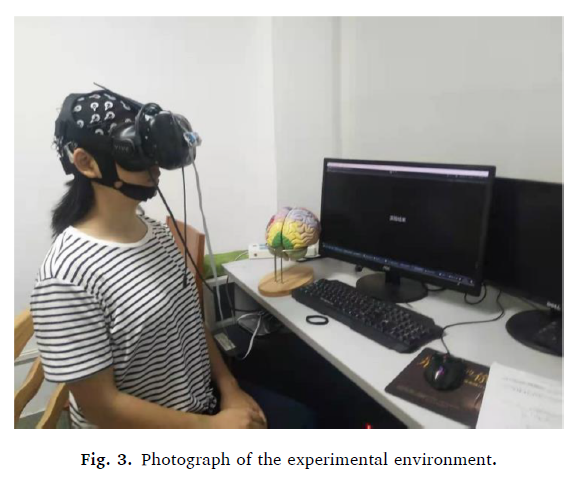
\includegraphics[width=0.4\linewidth]{Fig/F1.png}
		\qquad\qquad
		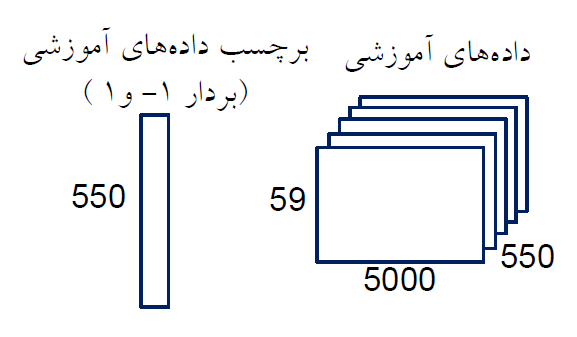
\includegraphics[width=0.4\linewidth]{Fig/F2.png}
	\end{center}

	We aim to train a MLP and RBF network in order to predict the label (sentiment of stimulus). This requires mapping our EEG recordings onto the feature space. A vital step is to extract and select features.

	\section{Feature Extraction}
	Two main categories of features are considered in this project:
	
	\subsection{Statistical time domain features}
	We will extract the following time domain features:
	\begin{enumerate}
		\item \textbf{Variance} \\
		We have developed a function called "calc\_feature\_var" to calculate the variance of each channel for each trial. The dimension of the output matrix will number of trials by number of channels.
		\begin{lstlisting}
			function result = calc_feature_var(data)
			
				% result = matrix of size trials by channel
				% calculating the variance of each channel
				ch_var = var(data, 0, 2);
				result = squeeze(ch_var)';
			
			end
		\end{lstlisting}
	
		\item \textbf{Amplitude Histogram}\\
		We first consider signal of a single trial from one channel. Given an amplitude range and number of bins, we will calculate the histogram for the number of bins. In a loop for all trials and all channels, we will do the same and finally will reshape the result to a 2D matrix where the first dimension demonstrate the trials and the second dimension demonstrates the amplitude histogram values for the number of bins and number of channels. Indeed size of the second dimension of the matrix will be $n\_bins \times n\_channels$. Here is the main part of the code, implemented for this feature:
		\begin{lstlisting}
			for i=1:n_trials
				for j=1:n_channels
					range = amp_range(1) <= data(j,:,i) & data(j,:,i) <= amp_range(2);
					selected_data = data(j, range, i);
					result(i,j,:) = histogram(selected_data, n_bins).Values;
				end
				fprintf("Step %d / %d ... \n", i, n_trials);
			end
			
			result = reshape(result, n_trials, []);
		\end{lstlisting}
	
		\item \textbf{AR model coefficients}\\
		In the context of time series analysis, an autoregressive (AR) model is a mathematical representation that describes the relationship between a variable and its past values. The AR model is defined by a set of coefficients that determine the influence of previous observations on the current value of the variable. \\\\
		Given the order, we will calculate the AR model coefficients for signal of all trials and all channels. We will use MATLAB built-in function called "ar()". The outcome matrix will have the dimension of (number of trials by (number of channels $\times$ order + 1)). Here is the main section of the code:
		\begin{lstlisting}
			for i=1:n_trials
				for j=1:n_channels
					AR_coef(i,j,:) = ar(data(j,:,i), order).A;
				end
				fprintf("Step %d / %d ... \n", i, n_trials);
			end
			
			AR_coef = reshape(AR_coef, n_trials, []);
		\end{lstlisting}
	
		\item \textbf{Form Factor (FF)}\\
		Form Factor for signal is calculate using the following formula:
		\begin{align*}
			FF = \frac{\sigma_{\ddot{s}} / \sigma_{\dot{s}}}{\sigma_{\dot{s}} / \sigma_{s}}
		\end{align*}
		Form Factor will be calculate using the following code:
		\begin{lstlisting}
			function FF = calc_feature_FF(data)
			
				sig_derivative_1 = diff(data, 1, 2);
				sig_derivative_2 = diff(sig_derivative_1, 1, 2);
				
				std_s_2 = squeeze(std(sig_derivative_2, 0, 2));
				std_s_1 = squeeze(std(sig_derivative_1, 0, 2));
				std_s_0 = squeeze(std(data, 0, 2));
				
				FF = (std_s_2 ./ std_s_1) ./ (std_s_1 ./ std_s_0);
				FF = FF';
				
			end
		\end{lstlisting}
		The output will of size (number of trials by number of channels).\\
		This form factor computation can be used to compare the variations or fluctuations in the signals at different points in time or under different conditions. By examining the relative changes in standard deviations, it provides insights into the shape or pattern of the signals and their evolution.
		
		\item \textbf{Correlation for signals of channels}\\
		Here is the main code for this section:
		\begin{lstlisting}
			for i=1:n_trials
				for j=1:n_channels
					for k=1:n_channels
						data1 = data(j,:,i);
						data2 = data(k,:,i);
						covariance = cov(data1, data2);
						cov_mat(i,j,k) = covariance(1,2);
					end
				end
				fprintf("Step %d / %d ... \n", i, n_trials);
			end
			
			cov_mat = reshape(cov_mat, n_trials, []);
		\end{lstlisting}
		In this code, for each trial we have calculate the covariance matrix for signal os channels which is of size (number of channels by number of channels). We will do the same for all trials. Finally we will flatten these covariance matrices and concatenate them for all trials.
	\end{enumerate}
	
	\subsection{Frequency domain features}
	The following frequency domains are considered for feature extraction:
	\begin{enumerate}
		\item \textbf{Maximum frequency}\\
		We first develop a function called "calc\_fft()" as following:
		\begin{lstlisting}
			function [f, amp] = calc_fft(signal, Fs)
			
				N = length(signal);
				sig_fft = fft(signal);
				amp = abs(sig_fft/N);
				amp = amp(1:N/2+1);
				amp(2:end-1) = 2*amp(2:end-1);
				f = Fs*(0:(N/2))/N;
				
			end
		\end{lstlisting}
		Then in another code, we will calculate the FFT of the signal and find the frequency that has the maximum amplitude:
		\begin{lstlisting}
			for i=1:n_trials
				for j=1:n_channels
					[f, data_fft] = calc_fft(data(j,:,i), fs);
					[~, maxIndex] = max(data_fft);
					result(i,j) = f(maxIndex);
				end
				fprintf("Step %d / %d ... \n", i, n_trials);
			end
		\end{lstlisting}
	
		\item \textbf{Average frequency}\\
		We will use the MATLAB built-in function to calculate the mean frequency for signal of each channel and each trial using the following code:
		\begin{lstlisting}
			for i=1:n_trials
				for j=1:n_channels
					result(i,j) = meanfreq(data(j,:,i), fs);
				end
				fprintf("Step %d / %d ... \n", i, n_trials);
			end
		\end{lstlisting}
	
		\item \textbf{Median frequency}\\
		We will use the MATLAB built-in function to calculate the mean frequency for signal of each channel and each trial using the following code:
		\begin{lstlisting}
			for i=1:n_trials
				for j=1:n_channels
					result(j,i) = medfreq(data(j, :, i), fs);
				end
				fprintf("Step %d / %d ... \n", i, n_trials);
			end
		\end{lstlisting}
	
		\item \textbf{Signal band power}\\
		For signal of each channel and each trial, we will calculate the power in 5 EEG bands consisting : delta, theta, alpha, beta and gamma. We will use MATLAB built-in function called "bandpower()" to do so. Here is the code developed for this section:
		\begin{lstlisting}
			freq_bands = [[0.1, 3]; [4, 7]; [8, 12]; [12, 30]; [30, 100]];
			
			for i = 1:n_trials
				for j = 1:n_channels
					for k = 1:n_bands
						band_power(i,j,k) = bandpower(data(j,:,i), fs, freq_bands(k,:));
					end
				end
				fprintf("Step %d / %d ... \n", i, n_trials);
			end
		\end{lstlisting}
		We note that the resulting output is a 2D matrix. The first dimension demonstrates the trials and the second dimension is (number of channels $\times$ number of bands).
	\end{enumerate}

	\subsection{Mapping data to feature space}
	Now that we have developed function to calculate different time and frequency domain features, we have developed a function called "create\_all\_feature\_space()", which utilize all of the previous functions to map raw data onto the feature space.\\\\
	The output of this code is a struct with following format:
	\pict{0.5}{F3}
	It can be seen that total number of extracted features is 5643!.\\\\
	Finally for ease of use in the following of the project, we will save the train and test data after mapping them to the feature space. It will takes about 30 minute to extract all of these features!
	
	\begin{lstlisting}
		Train_feature_space = create_all_feature_space(TrainData, fs, n_bins, amp_range, order);
		Test_feature_space = create_all_feature_space(TestData, fs, n_bins, amp_range, order);
		
		%% Save data
		
		save('../Data/Train_feature_space.mat', 'Train_feature_space');
		save('../Data/Test_feature_space.mat', 'Test_feature_space');
		
	\end{lstlisting}
	\section{Feature selection}
	In the previous part, we extracted 5643 features. Obviously we will not use all of these features. In this section we will discuss about feature selection procedure.
	
	\subsection{One dimensional Fisher score}
	Using the following function, we will calculate the fisher score for only one feature.
	\begin{lstlisting}
		function fisher = calculate_fisher(X, X1, X2)
		
			% Calculate class means
			mu_0 = mean(X);
			mu_1 = mean(X1);
			mu_2 = mean(X2);
			
			% Calculate class variances
			var_1 = var(X1);
			var_2 = var(X2);
			
			% Calculate Fisher score
			fisher = ((mu_0 - mu_1).^2 + (mu_0 - mu_2).^2) ./ (var_1 + var_2);
			
		end
		
	\end{lstlisting}
	We will pass the generate struct of feature space to a function called "". In this function we will calculate the fisher score for all fields of the input struct. Here is the main section of the code:
	\begin{lstlisting}
		for i = 1:numFields
			featureName = fields{i};
			featureValue = data.(featureName);
			
			% Calculate Fisher score for each column of the featureValue matrix
			fisherScores = zeros(1, size(featureValue, 2));
			for j = 1:size(featureValue, 2)
				column = featureValue(:, j);
				class1 = column(labels == -1);
				class2 = column(labels == 1);
				fisherScores(j) = calculate_fisher(class1, class2, column);
			end
			
			% Store feature name and Fisher scores in the struct
			featureScores(i).featureName = featureName;
			fisherScores(isnan(fisherScores)) = 0;
			featureScores(i).fisherScore = fisherScores;
			
			%         featureScores(i).fisherScore(isnan(featureScores(i).fisherScore)) = 0;
			
			% Sort the Fisher scores within each category (field)
			[~, sortedIndices] = sort(fisherScores, 'descend');
			featureScores(i).fisherScore = fisherScores(sortedIndices);
			featureScores(i).sortedIndices = sortedIndices;
	\end{lstlisting}
	This way, we have best features in each category alongside with best features considering all features. The output of this function we have the following format:
	\pict{0.5}{F4}
	Now we will consider two different methodologies for selecting best features one by one using fisher score.
	\begin{enumerate}
		\item Considering all 5643 features, we will calculate the fisher score then we sort them and choose the first "n" features. Here is the code for this section:
		\begin{lstlisting}
			n_feature = 100;
			train_indicies = featureScores(10).sortedIndices(1:n_feature);
			selected_feature_space = Train_data.all(:, train_indicies);
		\end{lstlisting}
	
		\item Another option is to choose the best "n" feature of each category. To do so, we have developed a function as follows:
		\begin{lstlisting}
			% Iterate over the fields of the input struct
			fields = fieldnames(data);
			for i = 1:numel(fields)
				fieldName = fields{i};
				
				% Retrieve the 2D array from the input struct
				array2D = data.(fieldName);
				
				% Select the desired rows based on the given indices
				Indices = fisherScores(i).sortedIndices(1:n);
				selectedCols = array2D(:, Indices);
				
				% Store the selected rows in the new struct
				selected_fearue_space = [selected_fearue_space selectedCols];
			end
		\end{lstlisting}
	\end{enumerate}

	\subsection{Bulky feature selection using Jscore}
	In the previous section, we selected feature one by one. This will not guarantee that the resulting combination of features will work well. In this section we consider different combination of features and evaluate them regarding J scores.\\\\
	We will calculate the J scores using the following code:
	\begin{lstlisting}
		function [J1, J2, J3] = calc_J_scores(X, X1, X2)
			
			% Calculate class means
			mu_1 = mean(X1, 1);
			mu_2 = mean(X2, 1);
			mu_0 = mean(X, 1);
			
			% Calculate between-class scatter matrix (S_b)
			S_b = (mu_1 - mu_0).' * (mu_1 - mu_0) + ...
			(mu_2 - mu_0).' * (mu_2 - mu_0);
			
			% Calculate within-class scatter matrices (S1 and S2)
			S1 = 1/size(X1, 1) * (X1 - mu_1).' * (X1 - mu_1);
			S2 = 1/size(X2, 1) * (X2 - mu_2).' * (X2 - mu_2);
			
			% Calculate within-class scatter matrix (S_w)
			S_w = S1 + S2;
			
			% Calculate J scores
			J1 = trace(S_b) / trace(S_w);
			J2 = det(S_b) / det(S_w);
			J3 = (mu_1' - mu_2').' * inv(S_w) * (mu_1' - mu_2');
			
		end
	\end{lstlisting} 
	Using the following code, we sort the combination of features regarding their J1 score:
	\begin{lstlisting}
		for i = 1:n_comb
		
			random_features = randperm(size(All_features, 2));
			currentCombination = random_features(:, 1:n_feature);
			
			% Extract the corresponding columns from the matrix
			selectedFeatureSpace = All_features(:, currentCombination); 
			class1 = selectedFeatureSpace(labels == -1, :);
			class2 = selectedFeatureSpace(labels == 1, :);
			
			[J1, J2, J3] = calc_J_scores(selectedFeatureSpace, class1, class2);
			featureScores.combination(i,:) = random_features(1:n_feature);
			featureScores.J1Score(i) = J1;
			featureScores.J2Score(i) = J2;
			featureScores.J3Score(i) = J3;
			
			fprintf("Step %d / %d ... \n", i, n_comb);
			
		end
		
		[~, J1_sortedIndices] = sort(featureScores.J1Score, 'descend');
		selected_features = All_features(:, featureScores.combination(J1_sortedIndices(1), :));
	\end{lstlisting}

	\subsection{Utilizing PSO in bulky feature selection using Jscore}
	It can be realized that the search space for different combination of features is quite wast where classic search algorithms won't perform well. Therefore we will use Particle Swarm Optimization aka PSO algorithm to find the best combination of features.\\\\
	Each particle in this algorithm represents the index of the selected feature. The fitness function is defined as follows:
	\begin{lstlisting}
		function out = PSO_calc_Jscore(data, feature_Indicies, labels)
		
			feature_Indicies = round(feature_Indicies);
			selectedFeatureSpace = data(:, feature_Indicies); 
			class1 = selectedFeatureSpace(labels == -1, :);
			class2 = selectedFeatureSpace(labels == 1, :);
			
			[JScore, ~, ~] = calc_J_scores(selectedFeatureSpace, class1, class2);
			
			out = 1/JScore;
			
		end
	\end{lstlisting}
	We aim to maximize the Jscore.
	The main code for PSO is as follows:
	\begin{lstlisting}
		options = optimoptions('particleswarm', 'SwarmSize', 50, 'MaxIterations', 100);
		
		% Define the objective function handle with extra parameters (X, k)
		objectiveFunction = @(feaure_indicies) PSO_calc_Jscore(Train_data.all, feaure_indicies, Trainlabels);
		
		% Run PSO to find cluster centroids
		numVariables = n_feature;
		lb = repelem(1, n_feature);
		ub = repelem(max_feature_num, n_feature);
		
		[bestFeatureIndicies, cost] = particleswarm(objectiveFunction, numVariables, lb, ub, options);
		
	\end{lstlisting}

	\section{Model Training}
	We will use two types of ANN models. Multi Layer Perceptron and Radial Based Function networks.
	\subsection{MLP}
	The following function implements an MLP (Multilayer Perceptron) training framework using k-fold cross-validation. It begins by initializing arrays to store the mean squared error (MSE) and accuracy for each fold. The cross-validation process is carried out using the cvpartition function, which splits the training data into k subsets. The function then iterates through each fold, creating an MLP model with the specified number of hidden neurons using the fitnet function. The training parameters are set, including disabling the training window display and configuring the division ratios for training, testing, and validation data. The MLP model is trained using the train function with the training data. \\\\
	Predictions are made on the validation set, and the MSE and accuracy are calculated by comparing the predictions with the actual values. The progress of the training process is printed for each fold. Finally, the function calculates the average MSE and accuracy across all folds and returns the trained network, average MSE, and accuracy. This approach provides a robust evaluation of the MLP model's performance and aids in assessing its ability to generalize to unseen data.
	
	\begin{lstlisting}
		function [net, avgMSE, accuracy] = train_MLP(n_hidden, trainX, trainY, k)
			% Initialize array to store MSE for each fold
			foldMSE = zeros(1, k);
			foldAccuracy = zeros(1, k);
			
			% Perform k-fold cross-validation
			cv = cvpartition(size(trainX, 1), 'KFold', k);
			for fold = 1:k
				% Get the indices for the current fold
				trainIndices = cv.training(fold);
				valIndices = cv.test(fold);
				
				% Get the training and validation sets for the current fold
				foldTrainX = trainX(trainIndices, :);
				foldValX = trainX(valIndices, :);
				foldTrainY = trainY(trainIndices);
				foldValY = trainY(valIndices);
				
				% Create the MLP model
				net = fitnet(n_hidden, 'trainlm');
				
				% Set the training parameters
				net.trainParam.showWindow = false;  % Disable training window display
				net.divideParam.trainRatio = 100/100;
				net.divideParam.testRatio = 0/100;
				net.divideParam.valRatio = 0/100;
				
				% Train the MLP model
				net = train(net, foldTrainX', foldTrainY);
				
				% Make predictions on the validation sets
				valPred = net(foldValX');
				
				% Calculate the MSE for the validation set
				foldMSE(fold) = mean((valPred - foldValY).^2);
				
				foldAccuracy(fold) = sum(round(valPred) == foldValY) / numel(foldValY);
				
				fprintf("Step %d / %d ... \n", fold, k)
			end
			
			% Calculate the average MSE across folds
			avgMSE = mean(foldMSE);
			accuracy = mean(foldAccuracy);
		
		end
	\end{lstlisting}

	\subsection{RBF}
	Once again, we repeat the k-fold cross validation procedure for RBF networks using the following code:
	\begin{lstlisting}
		function [net, avgMSE, accuracy] = train_RBF(n_hidden, sigma, trainX, trainY, k)
			% Initialize array to store MSE for each fold
			foldMSE = zeros(1, k);
			foldAccuracy = zeros(1, k);
			
			% Perform k-fold cross-validation
			cv = cvpartition(size(trainX, 1), 'KFold', k);
			for fold = 1:k
				% Get the indices for the current fold
				trainIndices = cv.training(fold);
				valIndices = cv.test(fold);
				
				% Get the training and validation sets for the current fold
				foldTrainX = trainX(trainIndices, :);
				foldValX = trainX(valIndices, :);
				foldTrainY = trainY(trainIndices);
				foldValY = trainY(valIndices);
				
				% Create the MLP model
				net = newrb(foldTrainX', foldTrainY, 0, sigma, n_hidden);
				
				% Make predictions on the validation sets
				valPred = net(foldValX');
				valPred(valPred >= 0) = 1;
				valPred(valPred < 0) = -1;
				
				% Calculate the MSE for the validation set
				foldMSE(fold) = mean((valPred - foldValY).^2);
				
				foldAccuracy(fold) = sum(valPred == foldValY) / numel(foldValY)
				
				fprintf("Step %d / %d ... \n", fold, k)
			end
			
			% Calculate the average MSE across folds
			avgMSE = mean(foldMSE);
			accuracy = mean(foldAccuracy);
			
		end
	\end{lstlisting}

	\subsection{Model Hyper parameters}
	In search of finding the best parameters for the RBF network which are the spread of the hidden neurons defined by "sigma" and also the number of hidden layers, we also tried PSO algorithm. Here is the fitness function used for this problem:
	\begin{lstlisting}
		function out = RBF_calc_Acc(data, model_param, Trainlabels, bestFeatureIndicies)
		
			sigma = model_param(1)
			n_hidden = round(model_param(2))
			
			k = 5;
			[~, ~, RBF_accuracy] = train_RBF(n_hidden, sigma, ...
			data(:, round(bestFeatureIndicies)), Trainlabels, k);
			
			out = 1/RBF_accuracy;
			
		end
	\end{lstlisting}
	Surprisingly, execution of this code took more than 7 hours!!! Based on the logged values, we estimated the best hyper parameters for our model and will use it in the next steps of the project.
	
	\section{Results}
	In this section we will report the results considering the best found models for each case.
	\subsection{Feature selection using Fisher score}
	Following the first methodology we discussed before, the best fisher score when considering all features can be seen below:
	\pict{1}{F5}
	In the following we will use top 100 features. Then we first train a MLP network with 3 hidden layers. Finally we will report the average accuracy. The feature space dimension for this section is 100.
	\begin{lstlisting}
		hiddenLayers = [10, 20, 10];
		k = 5;
		[MLP_net, avgMSE, accuracy] = train_MLP(hiddenLayers, selected_feature_space, Trainlabels, k);
	\end{lstlisting}
	The result can be seen below:
	\pict{0.6}{F6}
	The average accuracy is 71.6 \%.
	
	Now we train the RBF model. Regarding what we discussed about finding the best parameters for the RBF model, we decided to select the followings:
	\begin{lstlisting}
		n_hidden = 500;
		sigma = 1;
		k = 5;
		[RBF_net, RBF_avgMSE, RBF_accuracy] = train_RBF(n_hidden, sigma, selected_feature_space, Trainlabels, k);
	\end{lstlisting}
	The results can be seen below:
	\pict{0.6}{F7}
	It can be seen the this model doesn't perform well enough. The average accuracy is 51.45 \%.
	
	\subsection{Bulky Feature selection using J score}
	In this section, we used grid search to find the best "n" combination of features based on Jscore. Then we train the MLP network with 4 hidden layers containing 10, 20, 20 and 10 neurons. Then we evaluate it using 5-fold cross validation. Here are the results. The feature space dimension for this section is 200.
	\pict{0.6}{F8}
	The average accuracy is about 72\%.\\\\
	Then we generate the results for RBF network.
	\pict{0.6}{F9}
	Unfortunately, it can be seen that the RBF network has a poor performance.
	
	\subsection{Feature selection empowering PSO}
	Here we present the results generated when we select the features using PSO algorithm.\\\\
	Here are the results for the MLP network with 3 hidden layers containing 10, 20 and 10 neurons. The feature space dimension is 200.
	\pict{0.6}{F11}
	Here are the results for the RBF network:
	\pict{0.6}{F10}
	The average accuracy is 51\% which is relatively low.\\\\\\
	Also we note that all output labels are generated and stored in the corresponding directory for different methods regarding the given test data.
	
	\section{Limitations and future works}
	In this project we tried to predict the sentiment of the stimulus using recorded EEG data. Unfortunately, we failed to achieve an acceptably high accuracy. This is mainly because of the followings:
	\begin{itemize}
		\item \textbf{Features:}\\
		Only simple time domain and frequency domain features were considered in this project. Time-frequency features like wavelet transform can enhance the performance of the model as its more complicated feature. Another category of features which can be extremely effective is connectivity measures. In this article, the authors used Phase Lock Value as a measure of connectivity between electrodes. Phase Amplitude Coupling is a better measure of connectivity which can be used here.\\\\
		Since we are dealing with sentiments, we know that amygdala is involved in this task. We hypothesize that connectivity between amygdala and medial Prefrontal Cortex, encode the type of sentiment and we can search for the sentiment signature here. We note that since our recording are non-invasive EEG, we first have to localize our signals using methods like LORETA.
		
		\item \textbf{Models:}\\
		We used simple MLP and RBF models. These models are dealing with lots of hyper parameters e.g. number of hidden layers, number of neurons in each hidden layer, number of output neurons (one hot encoding, binary encoding), spread of neurons in RBF network, etc. The parameters can be set using optimization procedure. Higher performance can be achieved this way.\\\\
		Other models like logistic regression and Random Forest can be used for this classification task.
	\end{itemize}
	
\end{document}